% =============================================
% =============================================
% Document class: Article
\documentclass[ a4paper, twoside, 11pt]{article}
% Packages: LaTeX (Depth-1)
\usepackage[ vlined, linesnumbered, ruled]{algorithm2e}
\usepackage{ amsfonts, amsmath, amssymb, amsthm}
\usepackage[ titletoc, title]{appendix}
\usepackage{ bbm}
\usepackage{ color}
\usepackage{ dsfont}
\usepackage{ enumitem}
\usepackage{ graphicx}
\usepackage{ fancyhdr, float, fullpage}
\usepackage{ hyperref}
\usepackage{ lastpage, latexsym, lipsum}
\usepackage{ mathrsfs, mathtools, multicol}
\usepackage{ parskip}
\usepackage{ setspace, stmaryrd, subcaption}
\usepackage{ tabularx}
\usepackage{ wasysym}
\usepackage[ dvipsnames, table]{ xcolor}
\usepackage{ xfrac}
% Packages: LaTeX (Depth-2)
\usepackage{ epstopdf}

% =============================================
\topmargin 			= -1.6cm
\headheight 		= .90cm
\headsep 			= .80cm
\textheight 		= 24.0cm
\textwidth 			= 15.5cm
\oddsidemargin		= 0.cm
\evensidemargin 	= 0.cm

% =============================================
% =============================================
% Macros: Language
\newcommand{\define}{\triangleq}
\newcommand{\done}{\hfill $\square$}
%\newcommand{\eqCIRC}{\stackrel{\circ}{=}}
%\newcommand{\eqSTAR}{\stackrel{*}{=}}
\renewcommand{\epsilon}{\varepsilon}
\newcommand{\eg}{\textit{e.g.,\;}}
\newcommand{\egc}{\textit{e.g.:\;}}
\newcommand{\Eg}{\textit{E.g.,\;}}
\newcommand{\Egc}{\textit{E.g.:\;}}
\newcommand{\ie}{\textit{i.e.,\;}}
\newcommand{\iec}{\textit{i.e.:\;}}
\newcommand{\Ie}{\textit{I.e.,\;}}
\newcommand{\Iec}{\textit{I.e.:\;}}
\newcommand{\QED}{\hfill $\blacksquare$}
\renewcommand{\tilde}[1]{\widetilde{#1}}
\newcommand{\tsup}[1]{\ensuremath{^{\text{#1}}}}
\newcommand{\tsub}[1]{\ensuremath{_{\text{#1}}}}
\renewcommand{\vec}[1]{{\boldsymbol{#1}}}

% Macros: Optimization & Probability
\DeclareMathOperator*{\argmax}{arg\,max}
\DeclareMathOperator*{\argmin}{arg\,min}
\newcommand{\Exp}{\mathbb{E}}
\newcommand{\Indicate}[1]{ \IndFun \, \{ \, #1 \, \} }
\renewcommand{\Pr}{\mathbb{P}}
\newcommand{\Normal}{\mathcal{N}}
\newcommand{\std}{\text{std}}
\newcommand{\var}{\text{var}}

% Macros: Sets
\newcommand{\Complex}{\mathbb{C}}
\renewcommand{\emptyset}{\varnothing}
\newcommand{\Nat}{\mathbb{N}}
\renewcommand{\Re}{\mathbb{R}}
\newcommand{\ReNN}{{\Re}_{\geq 0}}
\newcommand{\ReSP}{{\Re}_{> 0}}
\renewcommand{\subset}{\subseteq}
\renewcommand{\supset}{\supseteq}
\newcommand{\Z}{\mathbb{Z}}
\newcommand{\ZNN}{{\Z}_{\geq 0}}

% Macros: Spacing & Other Commands
\newcommand{\fullcut}{\vspace{-\baselineskip}}
\newcommand{\fullskip}{\vspace{\baselineskip}}
\newcommand{\halfcut}{\vspace{-0.5\baselineskip}}
\newcommand{\halfskip}{\vspace{0.5\baselineskip}}
\renewcommand{\figurename}{Figura}
\renewcommand{\tablename}{Tabla}

% =============================================
% Sesion de Clase
\newcommand{\sesion}{01}
% Macros para definiciones, teoremas, etc
\newcounter{sesion}
\setcounter{sesion}{\sesion}
\theoremstyle{definition}
\newtheorem{definition}{Definici\'on}[sesion]
\newtheorem{example}[definition]{Ejemplo}
\newtheorem{exercise}[definition]{Ejercicio}
\newtheorem{note}[definition]{Nota}
\newtheorem{problem}[definition]{Problema}
\newtheorem{theorem}[definition]{Teorema}

% =============================================
% =============================================
\newcommand{\HeaderLine}{}
\newcommand{\FooterLine}{P\'agina \thepage ~de \pageref*{LastPage}}

\pagestyle{fancyplain}
\fancyhf{}

\rhead[]{\fancyplain{}{\HeaderLine}}
\lhead[\fancyplain{}{\HeaderLine}]{}
\lfoot[\fancyplain{}{\FooterLine}]{}
\rfoot[]{\fancyplain{}{\FooterLine}}

\renewcommand{\headrulewidth}{0.4pt}
\renewcommand{\footrulewidth}{0.4pt}
\renewcommand{\thefootnote}{\fnsymbol{footnote}}

% =============================================
% =============================================
\begin{document}
\allowdisplaybreaks

\begin{center}
\Large Control Autom\'atico (FIMCP-03905): Examen \sesion \\[1ex]
\small \textbf{A\~no:} 2016-2017 \qquad \textbf{T\'ermino:} II \qquad
\textbf{Instructor:} Luis I. Reyes Castro \qquad \textbf{Paralelo:} 02
\end{center}
\halfskip

\fbox{

\begin{minipage}[b][\height][t]{\textwidth}
\vspace{0.2 cm}

\begin{center}
\textbf{COMPROMISO DE HONOR}
\end{center}
\vspace{0.4 cm}

\scriptsize
{
Yo, \rule{60mm}{.1pt} al firmar este compromiso, reconozco que el presente examen est\'a dise\~nado para ser resuelto de manera individual, que puedo usar un l\'apiz o pluma y una calculadora cient\'ifica, \linebreak que solo puedo comunicarme con la persona responsable de la recepci\'on del examen, y que cualquier instrumento de comunicaci\'on que hubiere tra\'ido debo apagarlo. Tambi\'en estoy conciente que no debo consultar libros, notas, \linebreak ni materiales did\'acticos adicionales a los que el instructor entregue durante el examen o autorice a utilizar. Finalmente, me comprometo a desarrollar y presentar mis respuestas de manera clara y ordenada. \\

Firmo al pie del presente compromiso como constancia de haberlo le\'ido y aceptado. 
\vspace{0.4 cm}

Firma: \rule{60mm}{.1pt} \qquad N\'umero de matr\'icula: \rule{42mm}{.1pt} \hspace{0.5cm} \\[-0.8ex]

}

\end{minipage}

}

\textbf{Instrucciones:} Cada uno de los siguientes cinco problemas tiene un peso de 5 puntos, pero el examen ser\'a calificado sobre 20 puntos. Con esto en mente, escoja y resuelva cuatro problemas de entre los cinco problemas en este examen. Adicionalmente, indique en estas hojas cuales son los problemas que usted desee que se le califiquen. 

\halfskip

% =============================================
\begin{problem}
Encuentre la funci\'on de transferencia $G(s) \define \Theta_1(s) \, / \, T(s)$ para el siguiente sistema mec\'anico rotacional. 

\begin{figure}[htb]
\centering
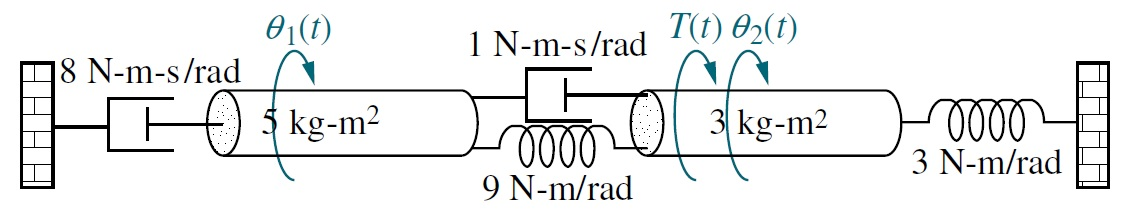
\includegraphics[ width = 0.66\textwidth]{fig_P2-30-A.jpg}
\end{figure}

\end{problem}
\vspace{\baselineskip}

% =============================================
\begin{problem}
Encuentre la funci\'on de transferencia $G(s) \define V_o(s) \, / \, V_i(s)$ asociada con el siguiente amplificador operacional. 

\begin{figure}[htb]
\centering
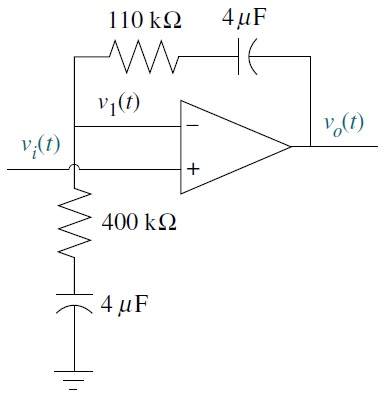
\includegraphics[ width = 0.36\textwidth]{fig_P2-22-A.jpg}
\end{figure}

\end{problem}
\vspace{\baselineskip}

% =============================================
\begin{problem}
Construya un modelo de espacio de estados para el sistema mec\'anico translacional mostrado en la figura de la siguiente p\'agina. 

\begin{figure}[htb]
\centering
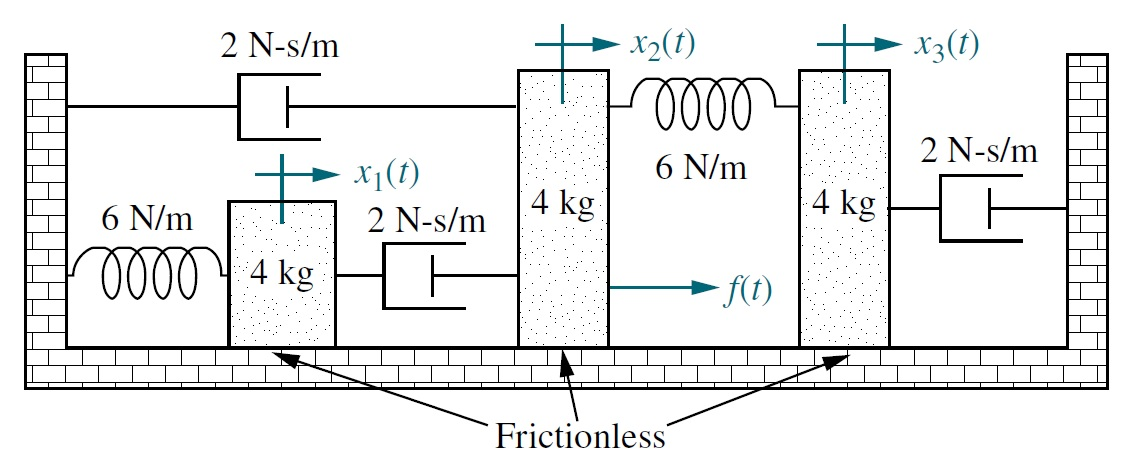
\includegraphics[ width = 0.68\textwidth]{fig_P2-27.jpg}
\end{figure}

\end{problem}
\vspace{\baselineskip}

% =============================================
\begin{problem}
Convierta el siguiente modelo de un sistema din\'amico representado como funci\'on de transferencia a un modelo de espacio de estados. 
\[
G(s) \, = \, 
\frac{ s^2 + 3s + 8 }{(s + 1) ( s^2 + 5s + 5 )}
\]

\end{problem}
\vspace{\baselineskip}

% =============================================
\begin{problem} Considere el siguiente modelo de las din\'amicas longitudinales de un caza-bombardero F4-E Phantom representado como modelo de espacio de estados. En este modelo, los estados son la aceleraci\'on normal, denotada $a_n(t)$, la velocidad del \'angulo de inclinaci\'on de la nariz, denotada $q(t)$, y el \'angulo del elevador horizontal, denotado $\delta_e(t)$. 
\begin{align*}
& \frac{d}{dt}
\left[ \begin{array}{c}
a_n(t) \\ q(t) \\ \delta_e(t)
\end{array} \right] \, = \, 
\left[ \begin{array}{ccc}
-1.70 & 50.7 & 263.4 \\
0.22 & -1.42 & -32 \\
0 & 0 & -14
\end{array} \right] 
\left[ \begin{array}{c}
a_n(t) \\ q(t) \\ \delta_e(t)
\end{array} \right]
+ \left[ \begin{array}{c}
-272.1 \\ 0 \\ 14
\end{array} \right] \delta_{com}(t)
\end{align*}

Con esto en mente, encuentre: 
\begin{itemize}
\item La matrices $C$ y $D$ para el caso cuando la salida es la aceleraci\'on normal $a_n(t)$. 
\item La funci\'on de transferencia: 
\[
G(s) \, \define \, \frac{A_n(s)}{\Delta_{com}(s)}
\]
%\item La matrices $C$ y $D$ para el caso cuando la salida es la velocidad del \'angulo de inclinaci\'on de la nariz $q(t)$. 
%\item La funci\'on de transferencia: 
%\[
%G(s) \, \define \, \frac{Q(s)}{\Delta_{com}(s)}
%\]
\end{itemize}

\end{problem}
\vspace{\baselineskip}

\end{document}
